\pagenumbering{arabic}
%\setcounter{page}{1}
\setcounter{chapter}{7}
\chapter{One Sample Confidence Intervals On a Proportion}
\index{Introduction}
\label{sec.matrix}
%start relabeling as 2.1 etc
\pagestyle{myheadings}  \markboth{\ref{sec.matrix}.
\titleref{sec.matrix}}{}
%\setcounter{equation}{0}

Perviously, we have introduced two types of confidence interval based on known and unknown variance. Moreover, confidence intervals are also applied to an unknown population proportion. For example, suppose we are interested the proportion of total number of left-handed students among all students who are currently studying at University of Toronto Mississauga. The question is: how do we know such the parameter which estimates the proportion of left-handed students at UTM? While, it is impossible to proceed it directly by counting both the total number of students and all left-handed students at UTM, due to the complexity and the total workload of that task. Then, we have to work with confidence intervals.\\

\noindent
Firstly, we take a random sample of students at UTM, then we calculate how many students are left-handed by dividing total number of left-handed students in that sample with total number of students in it, and denote the proportion as $\hat{p}$. Next we begin our confidence interval calculation to get a range of number with a certain level of confidence.\\

\noindent
Now let's begin with the proper definition of confidence interval on proportion.

\begin{definition}[One Sample Confidence Intervals On a Proportion]
We select a random sample of size $n$ from a population with \textbf{unknown} proportion $p$ of success. An approximate confidence interval for \textbf{p} is: \[ p = \hat{p}  \pm z_{\frac{\alpha}{2}} \cdot \sqrt{\frac{\hat{p}(1 - \hat{p})}{n}}, \text{ where $\hat{p} = \frac{\text{number of observations satisfying the criteria}}{n}$.}\]
In addition, $n$ is the sample size.\\
To apply this confidence interval, there are $3$ conditions that we need to guarantee:
\begin{itemize}
	\item $1$. Random sample;
	\item $2$. Independent and identically distributed Bernoulli trails;
	\item $3$. We have a large chosen sample size ($n\hat{p} \ge 10$ and $n(1-\hat{p}) \ge 10$).
\end{itemize}
\end{definition}

\noindent
A good way to understand confidence interval is visualization. Now, suppose we have a valid estimation $\hat{p}$. After the entire procedure of confidence interval, our population proportion ($p$) should be as the following number line shows:\\

\begin{center}
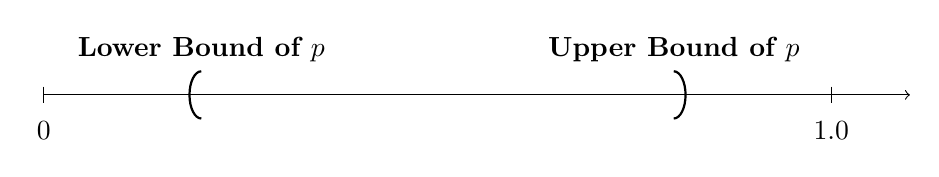
\begin{tikzpicture}
  \draw[->] (0,0) -- (11,0);
  \foreach \x in {0, 1.0} {
    \draw[shift={(\x*10,0)},color=black] (0pt,3pt) -- (0pt,-3pt);
    \draw[shift={(\x*10,0)},color=black] (0pt,-6pt) node[below] {\x};}
  \draw[thick] (2.0,-0.3) arc (270:90:0.15cm and 0.3cm);
  \node[above] at (2.0,0.3) {\textbf{Lower Bound of $p$}};
  \draw[thick] (8.0,-0.3) arc (-90:90:0.15cm and 0.3cm);
  \node[above] at (8.0,0.3) {\textbf{Upper Bound of $p$}};
\end{tikzpicture}
\end{center}

\noindent
Remember that your final answer of the range of $p$ must between $0$ and $1$, since we are working with proportion.\\

\noindent
\textbf{Summery about One Sample Confidence Intervals}

\noindent
We have introduced one sample confidence interval under three different cases: given population variance, unknown population variance and unknown population proportion. All the material of one sample confidence interval comes from chapter $6, 7, 8$, which seems like you to remember a lot. However, the reason why we give this summery is to help you to remember the basic skeleton of one sample confidence interval. Let's revisit the three distinct types of confidence interval:

\begin{itemize}
	\item 1. For given population variance, we have: $\bar{x}  \pm z_{\frac{\alpha}{2}} \cdot \frac{\sigma}{\sqrt{n}};$
	\item 2. For unknown population variance, we have: $\bar{x}  \pm t_{\frac{\alpha}{2}} \cdot \frac{s}{\sqrt{n}};$
	\item 3. To estimate population proportion, we have: $p = \hat{p}  \pm z_{\frac{\alpha}{2}} \cdot \sqrt{\frac{\hat{p}(1 - \hat{p})}{n}}.$
\end{itemize}

\noindent
The question is: what is the similarity between the three distinct types of confidence interval? You may have already noticed that the confidence intervals above are all follow such a skeleton that $\bar{x}$ plus or minus its margin of error (different between each type of C.I.).\\ 

\noindent
If we keep questioning ourselves that how the margin of error comes from, you will catch the pattern. The margin of error contains reference distribution and the standard deviation of $\bar{x}$ under its reference distribution. Let's analyze each type of confidence interval to prove my statement is true:\\

\noindent
The first type (given population variance) confidence interval is quite easy to recognize. Recall chapter $3$: The Central Limit Theorem, we state that $\bar{x} \sim N(\mu, \frac{\sigma^2}{n})$, which is how reference distribution comes from with given population variance. To get the standard deviation of $\bar{x}$, we simply take the square root of the variance, then $s_{\bar{x}} = \frac{\sigma}{\sqrt{n}}$. Finally, we multiply reference distribution at the point $\frac{\alpha}{2}$ with the standard deviation of $\bar{x}$ under normal distribution to get the margin of error.\\

\noindent
The second type (unknown population variance) confidence interval is similar to the first type, but the reference distribution is t-distribution instead of normal distribution. In chapter $7$, we introduced the calculation of sample variance ($s^2$) to estimate population variance ($\sigma^2$), and $s^2$ is an unbiased estimator of $\sigma^2$ (the proof of this statement is in STA260, in this course we can assume it freely). In chapter $2$, we defined that $T = \frac{\bar{x} - \mu}{(\frac{s}{\sqrt{n}})} \sim t_{n-1},$ then the term $\frac{s}{\sqrt{n}}$ (verify this by yourself as an extra exercise) is the standard deviation of $\bar{x}$ under t-distribution with $n-1$ degrees of freedom. Finally, we multiply multiply reference distribution at the point $\frac{\alpha}{2}$ with the standard deviation of $\bar{x}$ under t-distribution to get the margin of error.\\

\noindent
The third type (estimate population proportion) confidence interval is slightly harder to identify. Recall chapter $4$ that we can approximate binomial distribution by normal distribution. Suppose that a random variable $X \sim Binomial(n,p)$, then the random variable $X \sim N(np, np(1-p)).$ From chapter $4$, we know that $\hat{p} \sim N(\mu_{\har{p}} = p, \sigma_{\hat{p}}^{2} = \frac{p(1-p)}{n})$. Trivially, the standard deviation of $\hat{p}$ is $\sqrt{\frac{p(1-p)}{n}}$, since we don't know the value $p$ and use $\hat{p}$ to estimate that. Then, standard deviation of $\hat{p}$ is $\sqrt{\frac{\hat{p}(1-\hat{p})}{n}}$. Finally, by multiplying the reference distribution and standard deviation, we get the margin of error of the confidence interval.\\

\noindent
\textbf{Conclusion About One Sample Confidence Intervals}

\noindent
If you follow the skeleton below, one sample confidence interval will become easier:

\begin{itemize}
	\item 1. Identify what type of one sample confidence interval to use from given information;
	\item 2. Construct your confidence interval that fits the circumstance which you are facing, it either going to be $\bar{x}  \pm M.E.(\bar{x})\text{ or } \hat{p}  \pm M.E.(\hat{p});$
	\item 3. Check the validity of your final answer. For example, the range of $p$ must between $0$ and $1$.
	\item 4. Clearly state your final conclusion: we have a certain percentage of confidence to guarantee that the value of the chosen sample is between its lower bound and upper bound.
\end{itemize}
